\documentclass[10pt]{article}
\usepackage[spanish]{babel}
\usepackage{graphicx}
\usepackage[usenames,dvipsnames]{xcolor}
\usepackage{color}

%codigos: \begin{abstract} \end{abstract} es resumen
%nueva pagina \newpage
%colores predefinidos : white, black, red, green, blue, cyan, magenta, yellow
%\textcolor{blue}{text}
%\color{blue!20!black!30!green}{Prueba} mezcla de colores, conviene manejar solo 2 colores, es mas manejable



\begin{document}
{\centering
{\Large{Escuela Superior Polit\'ecnica del Litoral\\Facultad de Ingenier\'ia en Electricidad y Computaci\'on\\}}
\vspace{0.6in}

\includegraphics[scale=0.5]{espol.png}\\
\vspace{0.8in}
{\LARGE \textbf{\color{blue}{Lenguajes de Programaci\'on\\\vspace{0.3in}Experiencias de cada lenguaje}}\\
\vspace{0.5in}

%------------------------------------------------------------------------------------------%
\newpage
\tableofcontents

%------------------------------------------------------------------------------------------%
\newpage
\begin{flushleft}
\section{Android}
\vspace{0.5in}
\begin{abstract}
\vspace{0.3in}
\large{Este es el primer trabajo de lenguajes de programaci\'on,para el cual las indicaciones fueron las de realizar un proyecto de aplicaci\'on m\'ovil, mas espec\'ifico en Android.\\
Hubieron algunas dificultades al principio, era algo nuevo para todos, a\'un no ten\'iamos clara la idea de lo que se har\'ia.\\
Entre algunas ideas, finalmente surgi\'o MY TWIN, algo que realmente nos pareci\'o novedoso y con alguna utilidad que se puede agregar a un dispositivo m\'ovil.\\
Se trabajo bastante con los recursos del tel\'efono y se hizo mucho \'enfasis en la proyecci\'on de tener un dispositivo con todo personalizado.}
\end{abstract}
\begin{center}
\vspace{0.5in}

\includegraphics[scale=0.7]{logo}
\end{center}
\end{flushleft}

%------------------------------------------------------------------------------------------%
\newpage
\begin{flushleft}
\subsection{Introducci\'on}

\normalsize
MY TWIN una aplicaci\'on dirigida a toda clase de usuario mediante la cual podr\'as crear tu propio avatar, el cual se convertir\'a en tu asesor personal de tareas.

Una aplicaci\'on la cual jugar\'a con los estados de \'animo de tu avatar, los cuales estar\'an definidos por las diferentes tareas que cumplir\'a. Esto es que la aplicaci\'on no solo ser\'a para entretenimiento tendr\'a una funcionalidad que buscar\'a ayudar al usuario de una manera diferente, entretenida y personalizada.\\

\subsection{Idea}
\subsubsection{Problem\'atica}
Muchas veces tenemos nuestro celular o cualquier dispositivo m\'ovil en al cual podemos programar para que nos notifique o nos recuerde algunas tareas, pero eso es todo lo que hace.\\
Buscabamos entonces una funcionalidad extra al tel\'efono y que a la vez sea agradable al ususario.\\
Todo comenz\'o con una lluvia de ideas, donde algunas fueron muy simples y de poca utilidad y otrass en cambio eran muy complicadas y sin prestar el mayor benefecio, as\'i finalmente surgi\'o My Twin, idea que nos agrad\'o por que era posible de llevar a la realidad y adem\'as mejorar\'ia la funcionalidad de nuestro dispositivo m\'ovil.\\
My Twin como un entretenido gemelo virtual.\\
\vspace{0.3in}
\begin{center}
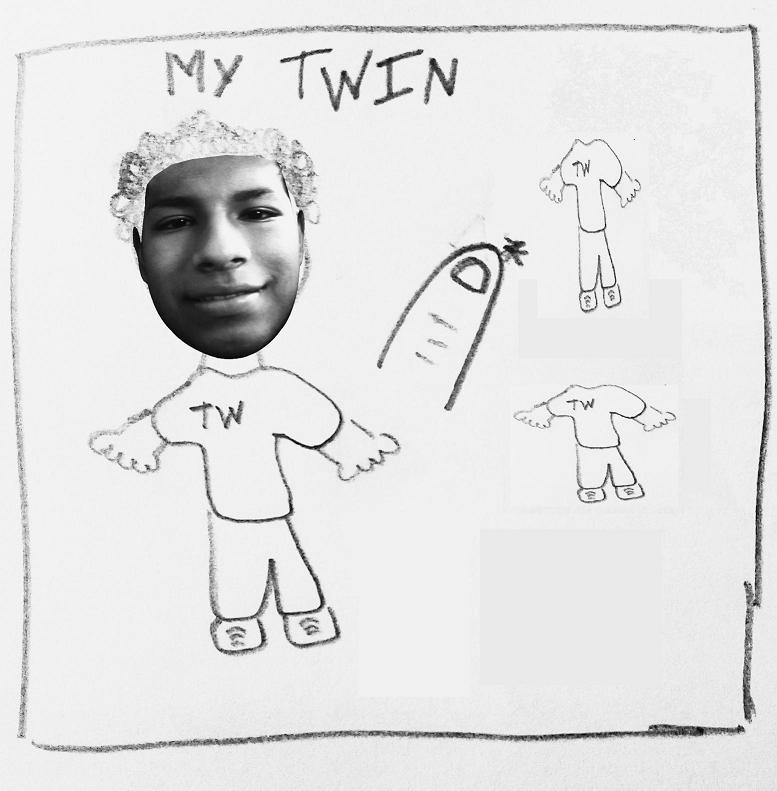
\includegraphics[scale=0.35]{bosquejoI1}
\end{center}

\end{flushleft}
}

%------------------------------------------------------------------------------------------%
\newpage
\begin{flushleft}
\subsubsection{Dise\~no}
El primer borrador fue trabajado en hojas con dibujos a mano, debido a que My Twin no era una sola pantalla est\'atica, sino que tiene algunas pantallas en la cual va cada una de las funciones.\\
Se dibujo algunos probables dise\~nos hasta llegar al que se tom\'o como modelo el siguiente.\\
\vspace{0.3in}
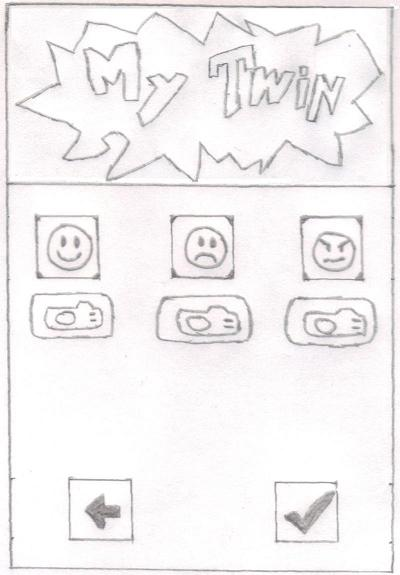
\includegraphics[scale=0.5]{Twin1}
\hspace{0.2in}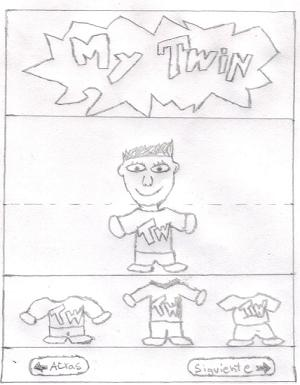
\includegraphics[scale=0.75]{Twin2}\vspace{0.2in}
\begin{center}
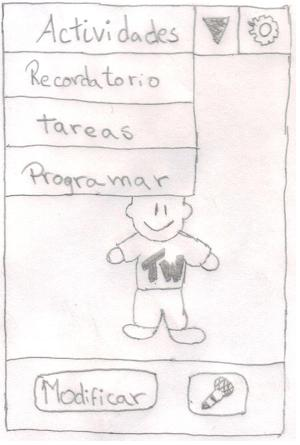
\includegraphics[scale=0.6]{Twin3}
\end{center}


\end{flushleft}


%------------------------------------------------------------------------------------------%
\newpage
\begin{flushleft}
\subsection{My Twin}
\subsubsection{Descripci\'on General}
\vspace{0.2in}
My Twin es una aplicaci\'on para dispositivo m\'ovil: \\\vspace{0.2in}\textbf{My Twin es divertido y original.\\
\vspace{0.1in}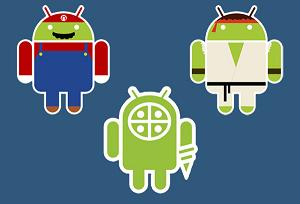
\includegraphics[scale=0.6]{3.jpg}\\
\begin{center}
\vspace{0.1in}My Twin es realista.\\
\vspace{0.1in}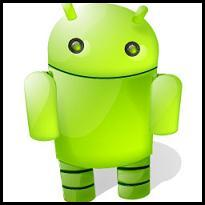
\includegraphics[scale=0.6]{droid.jpg}\\
\end{center}
\begin{flushright}
\vspace{0.1in}My Twin es amigable con el usuario.\\
\vspace{0.1in}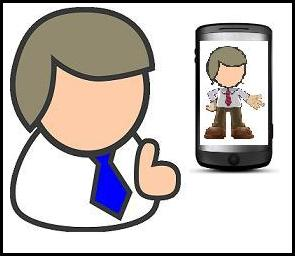
\includegraphics[scale=0.6]{amigableU.jpg}\\
\end{flushright}
}


\end{flushleft}

%------------------------------------------------------------------------------------------%
\newpage
\begin{flushleft}
\subsection{Funcionamiento (Manual de Usuario)}
\subsubsection{Pantalla Principal}

Pantalla Principal de My Twin, presionando en entrar, nos llevar\'a a la siguiente pantalla, si no tenemos aun creado el Twin, iremos a la pantalla de crear Twin, si ya lo tenemos, iremos directamente a la pantalla donde esta el menu y nuestro Twin.

\begin{center}
\vspace{0.1in}Pantalla Principal de inicio.\\
\vspace{0.1in}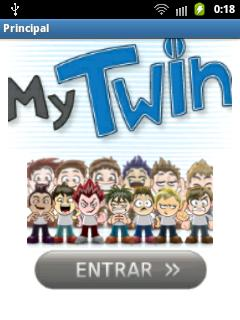
\includegraphics[scale=0.7]{PPrincipal}\\
\end{center}

\subsubsection{Creaci\'on de Twin}
Estas son las dos pantallas de creaci\'on del gemelo virtual, la primera es donde realizamos las fotos para la cara, d\'andole as\'i realismo; la segunda es para escoger un cuerpo, el cual le pone el lado original y divertido,donde todo es personalizable. \\
\begin{center}
\vspace{0.1in}
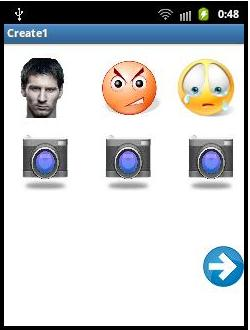
\includegraphics[scale=0.7]{create1.jpg}
\hspace{0.4in}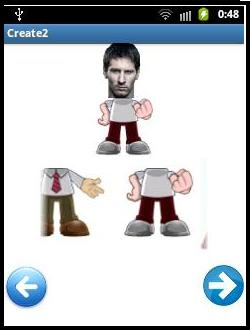
\includegraphics[scale=0.7]{create2.jpg}
\end{center}



\newpage
\subsubsection{Menu Tareas}
Luego de tener creado nuestro gemelo virtual, podemos ver el menu de tareas, el cual ser\'a la pantalla que veremos cada vez que entremos a la aplicaci\'on, el funcionamiento es sencillo, cuando vemos el menu se muestra en claras palabras lo que encontraremos al ingresar ah\'i.\\\vspace{0.2in}
\textbf{Tareas:} Nos llevar\'a a la pantalla de tareas, en la cual podremos programar los recordatorios de manera personalizada.\\\vspace{0.1in}
\textbf{Modificar:} Nos llevar\'a de regreso a la pantalla de creaci\'on de Twin, para que podamos realizar las modificaciones que queremos.\\\vspace{0.1in}
\textbf{Programar:} Nos permitir\'a programar el tel\'efono para casos especiales, como por ejemplo el ahorro de energ\'ia.\\

\begin{center}
\vspace{0.4in}
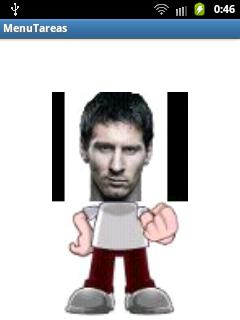
\includegraphics[scale=0.8]{MenuTareas1.jpg}
\hspace{0.4in}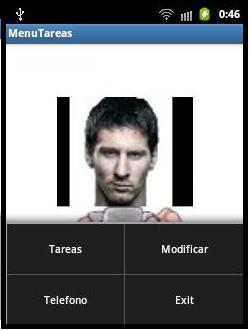
\includegraphics[scale=0.8]{MenuTareas2.jpg}
\end{center}

\newpage
\subsubsection{Nueva Tarea}
Aqu\'i podemos ver tres botones que hacen referencia al sonido, adem\'as de un reloj.\\
El funcionamiento es muy sencillo. En el reloj ponemos la hora que queremos establecer para recordar y los botones de grabacion funcionan así: uno para grabar, otro para detener y otro para reproducir la grabaci\'on.\\
Es importante recalcar que sin grabaci\'on no se puede avanzar, porque esto es parte del objetivo de buscar la originalidad, por esto es necesario que la tarea la recuerde con nuestra voz.\\
La otra parte importante es que podemos realizar tantas grabaciones como queramos, pues solo se escoger\'a la \'ultima, como parte de darle facilidad al ususario para que no tenga que iniciar el proceso nuevamente, esto se realiza de una manera sencilla en el mismo momento.\\

\begin{center}
\vspace{0.4in}
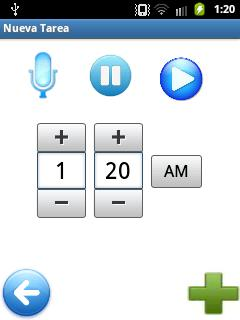
\includegraphics[scale=0.8]{NuevaTarea1.jpg}
\hspace{0.4in}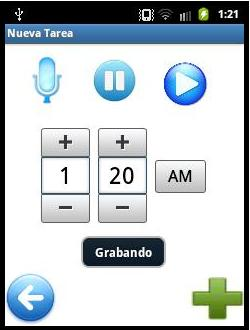
\includegraphics[scale=0.8]{NuevaTarea2.jpg}
\end{center}


\newpage
\subsubsection{Programar}
Esta funci\'on de la aplicaci\'on nos permite manejar recursos mas internos del dispositivo m\'ovil, de modo que se pueda programar su funcionamiento y manejarlo con un tiempo definido.\\

\begin{center}
\vspace{0.4in}
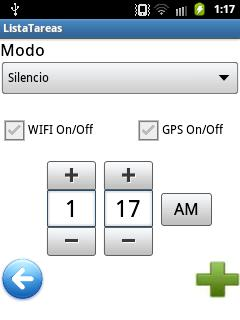
\includegraphics[scale=0.8]{Programar1.jpg}
\end{center}

\newpage
\subsection{Conclusiones}
Consideramos que logramos una aplicaci\'on completa que rompe la monoton\'ia de alarmas con tonos ruidosos
por una grabaci\'on de voz realizada por el usuario; aparte de eso la aplicaci\'on nos permite controlar los recursos 
b\'asicos del telefono.
\subsubsection{Experiencias Generales}
Realizar este trabajo no ha sido algo f\'acil, tuvimos varios inconvenientes. Al principio no encontrabamos la idea que nos ayudar\'ia a realizar este proyecto, luego vimos que este entorno de trabajo era diferente a lo que anteriormente hemos realizado, lo bueno es que contabamos con buenas bases de programaci\'on lo cual facilitaba un poco el entendimiento de lo nuevo que estabamos por ver.\\
En general el grupo siempre estuvo en contacto, de ese modo siempre se avanzaba en el trabajo, algunas veces tuvimos que trabajar hasta muy tarde por la noche, pero, a\'un as\'i vali\'o la pena, porque el trabajo se present\'o completo cumpliendo las expectativas que ten\'iamos acerca de la aplicaci\'on, adem\'as que ayud\'o a unir al grupo en amistad, pues cada problema que se presentaba se resolv\'ia realizando una reuni\'on ya sea f\'isicamente o por medio del internet.\\
Muchas de las cosas hubo que investigarlas puesto que esta era una experiencia nueva para todos y ninguno ten\'ia el conocimiento de lo que realizar\'iamos. Para resolver de manera mas eficiente, cada uno investigaba una parte y luego en reuni\'on expresabamos lo que hab\'iamos encontrado; en conjunto aprendimos cada uno de la experiencia del otro y de la informaci\'on que le toco buscar.\\
El entorno de trabajo para Android fue un poco complicado, pero sirvi\'o para darnos un empuje a lo que ser\'ian los otros proyectos de la materia, pudimos ver desde otra perspectiva la programaci\'on utilizando otras herramientas para trabajar; el hecho de tener exposiciones peri\'odicas del avance del proyecto nos presionaba precisamente a eso, que el proyecto estuviese en marcha, de este modo no nos atrasamos ni en terminar el trabajo ni en presentarlo.\\
\vspace{0.1in}Finalmente toda experiencia es y ha sido enriquecedora desde el punto de vista de conocimiento.

\end{flushleft}



\end{document}